\section{User Study}
\subsection{Introduction}

To validate the effectiveness of our system, we conducted a Within-Subjects User Study. The study was designed to demonstrate the system's capability for research applications. We aimed to select a study that would both showcase the system's capabilities and contribute novel insights to the field. We settled on a study to test user performance with volumetric displays under two different conditions as outlined below.

\subsection{Experimental Variables}

We aimed to test the following two hypotheses:
\begin{itemize}
    \item \textbf{H1}: Is there a difference in task performance when interacting with the volumetric display in 3D as opposed to 2D?
    \item \textbf{H2}: Is there a difference in task performance when interacting with the volumetric display directly with hands as opposed to via teleoperation?
\end{itemize}

To test these hypotheses, we designed a 2x2 within-subjects experiment. Our two independent variables were:
\begin{itemize}[itemsep=-0.25em]
    \item \textbf{Perspective:} \texttt{Static} vs. \texttt{Tracker}. This variable controls whether the system uses a tracking mechanism to create the illusion of a 3D volumetric display (\texttt{Tracker}) or a fixed perspective on a standard monitor (\texttt{Static}), as shown in Fig~\ref{fig:static-vs-tracker}. This tests \textbf{H1}.

    \begin{figureBox}[label={fig:static-vs-tracker}, width=0.8\linewidth]{2D \& 3D}
        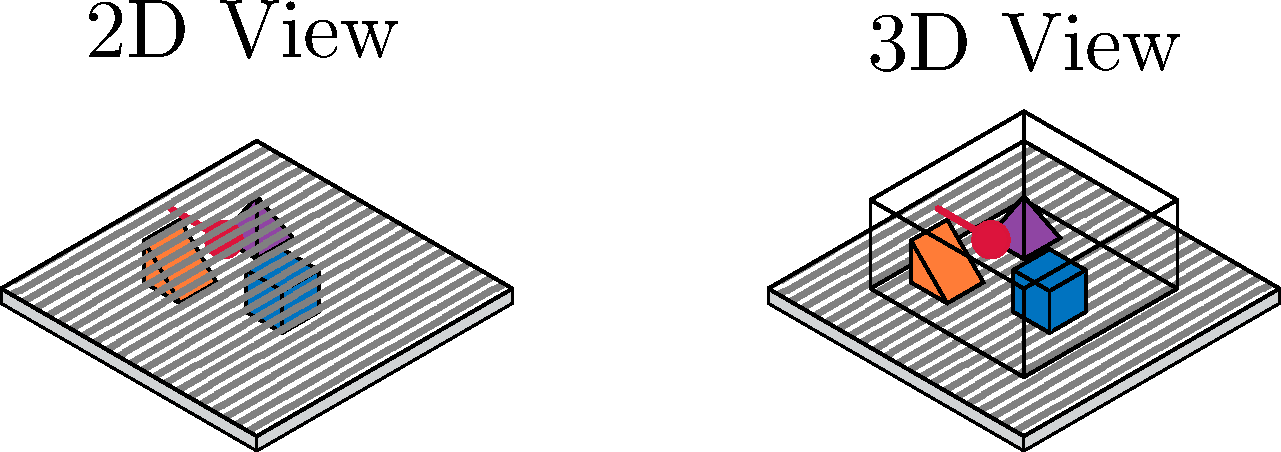
\includegraphics[width=0.8\linewidth]{./implementation/figures/2D-vs-3D.pdf}
    \end{figureBox}

    \item \textbf{Interaction Offset:} Offset vs. No Offset. This variable controls whether the display is directly in front of the participant or offset by a fixed amount, as shown in Fig~\ref{fig:direct-vs-offset}. This tests \textbf{H2}.

    \begin{figureBox}[label={fig:direct-vs-offset}, width=0.8\linewidth]{Direct \& Offset Interaction}
        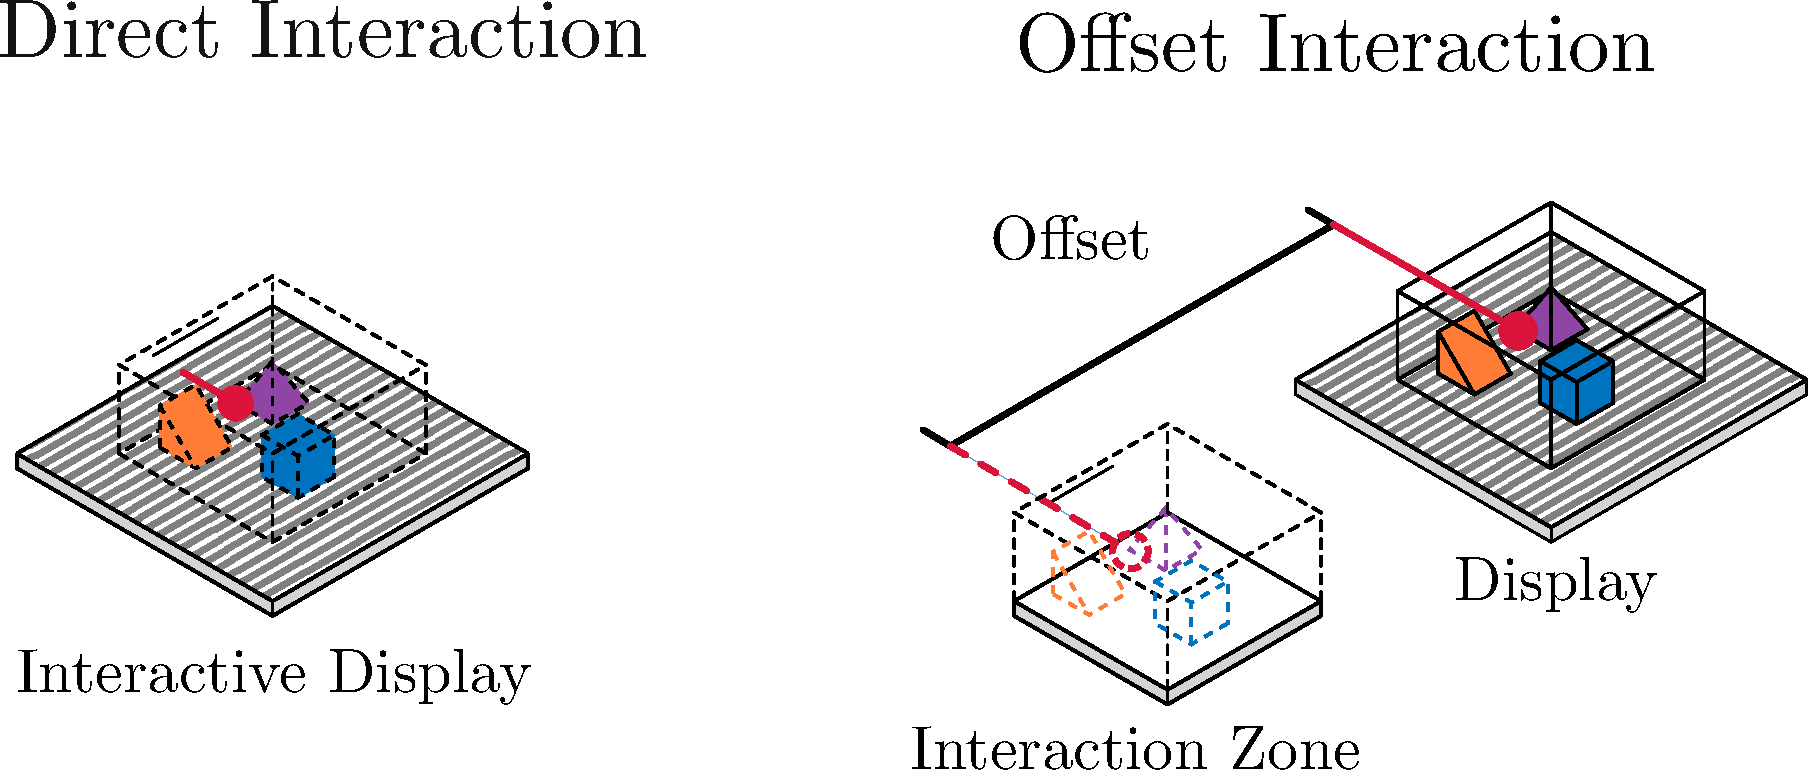
\includegraphics[width=0.8\linewidth]{./implementation/figures/direct-vs-offset.pdf}
    \end{figureBox}
\end{itemize}

We controlled for the following variables during the study:
\begin{itemize}
    \item \textbf{Tasks:} We ensured that the five tasks were identical in each condition.
    \item \textbf{Device Calibration:} The positions of the participant, the tracking camera, and the interaction zone were kept consistent across conditions, as shown in Fig~\ref{fig:test-setup}. When using an offset position, another display was placed where the original display was to maintain consistent tracking.
    \item \textbf{Lighting:} We maintained consistent lighting conditions in the room, as lighting significantly impacts the system's tracking quality.
\end{itemize}

\begin{figureBox}[label={fig:test-setup}, width=0.8\linewidth]{Test Setup}
    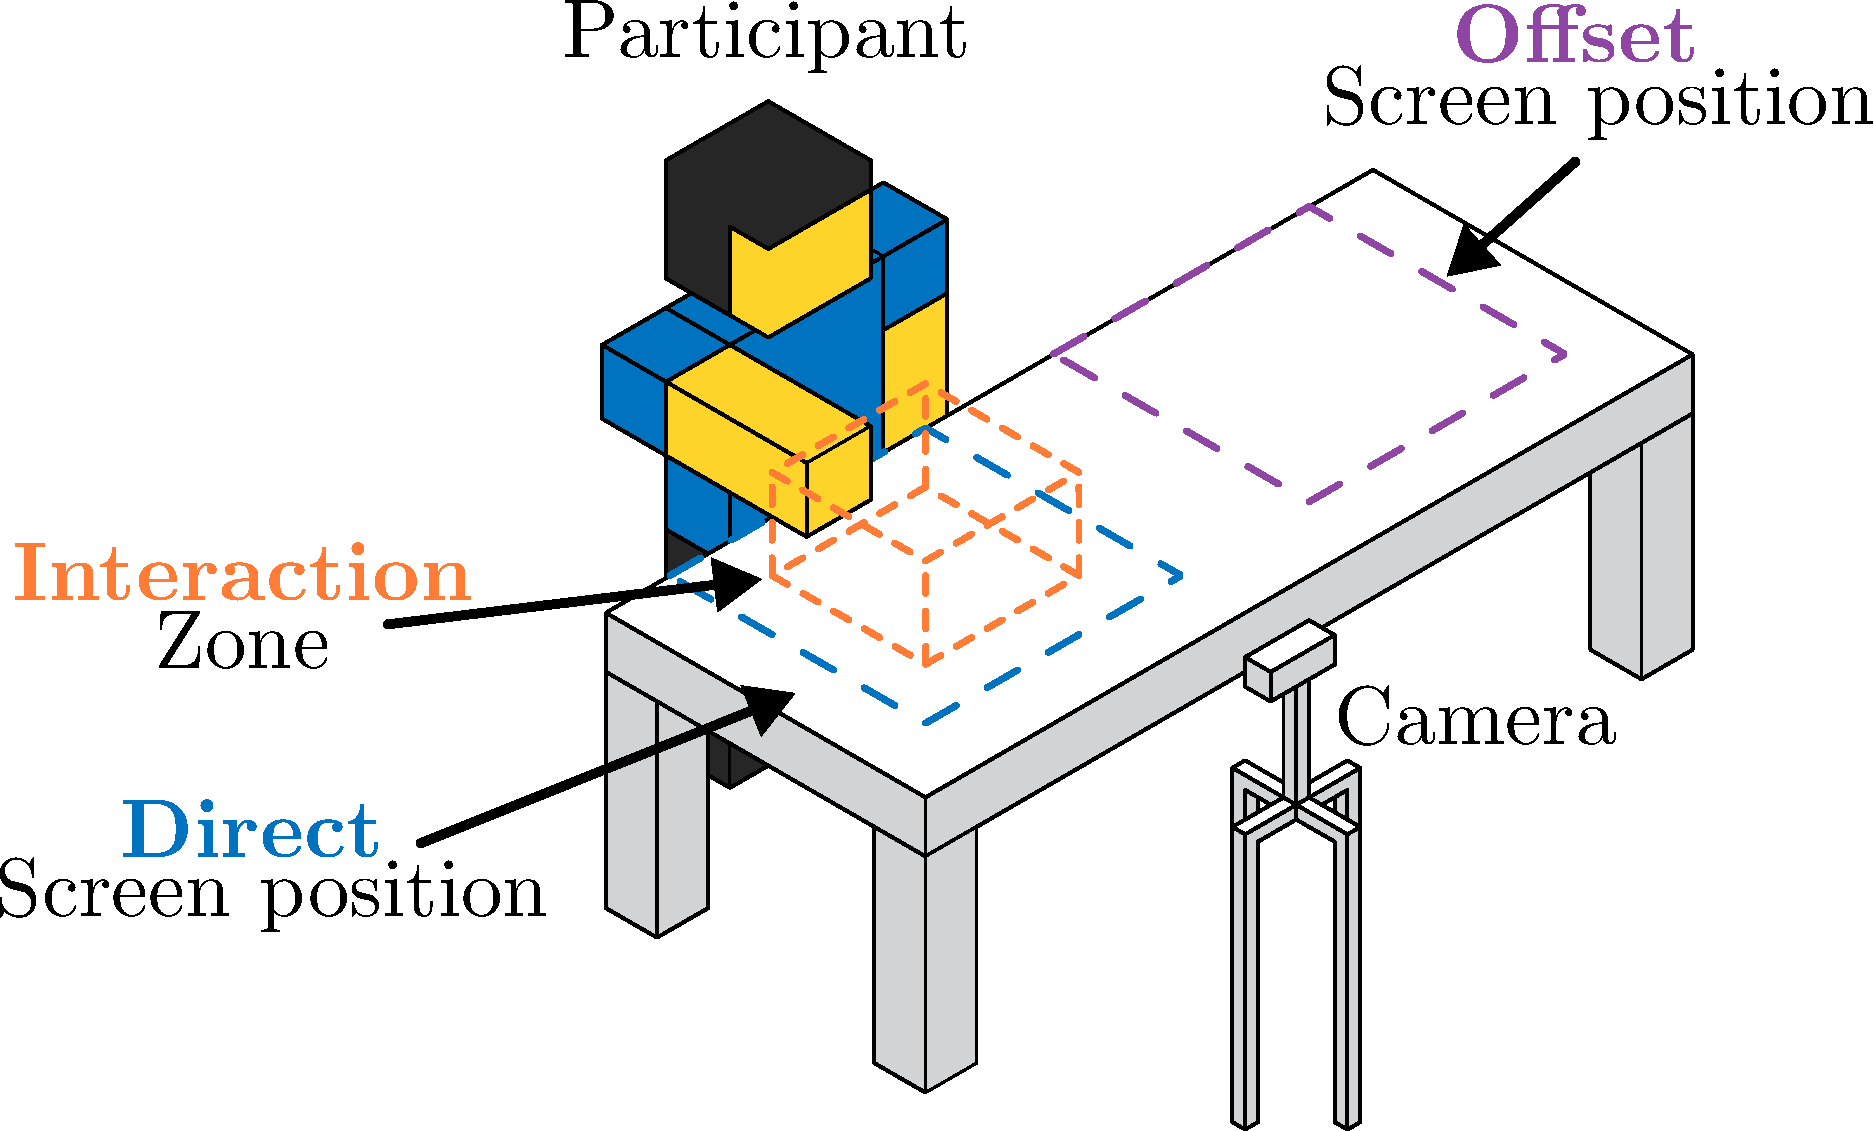
\includegraphics[width=0.8\linewidth]{./implementation/figures/test-setup.pdf}
\end{figureBox}

\subsection{Tasks}
In each of the four combinations of conditions, participants must complete the same five tasks in the same order. The tasks are designed to be simple to understand but challenging to complete. They were crafted so that, from any perspective, the components would visually overlap. \\

To complete a task, participants must trace the path between points using their index and middle fingers in the order presented by the simulator. A green point indicates a completed segment, an orange point represents the next segment to be completed, and a red point shows the current position of the participant's hand. Each time a task segment is completed, the colors update accordingly. An example of a completed task can be seen in Fig~\ref{fig:task-example}.

\begin{figureBox}[label={fig:task-example}, width=0.8\linewidth]{Completing a Task}
    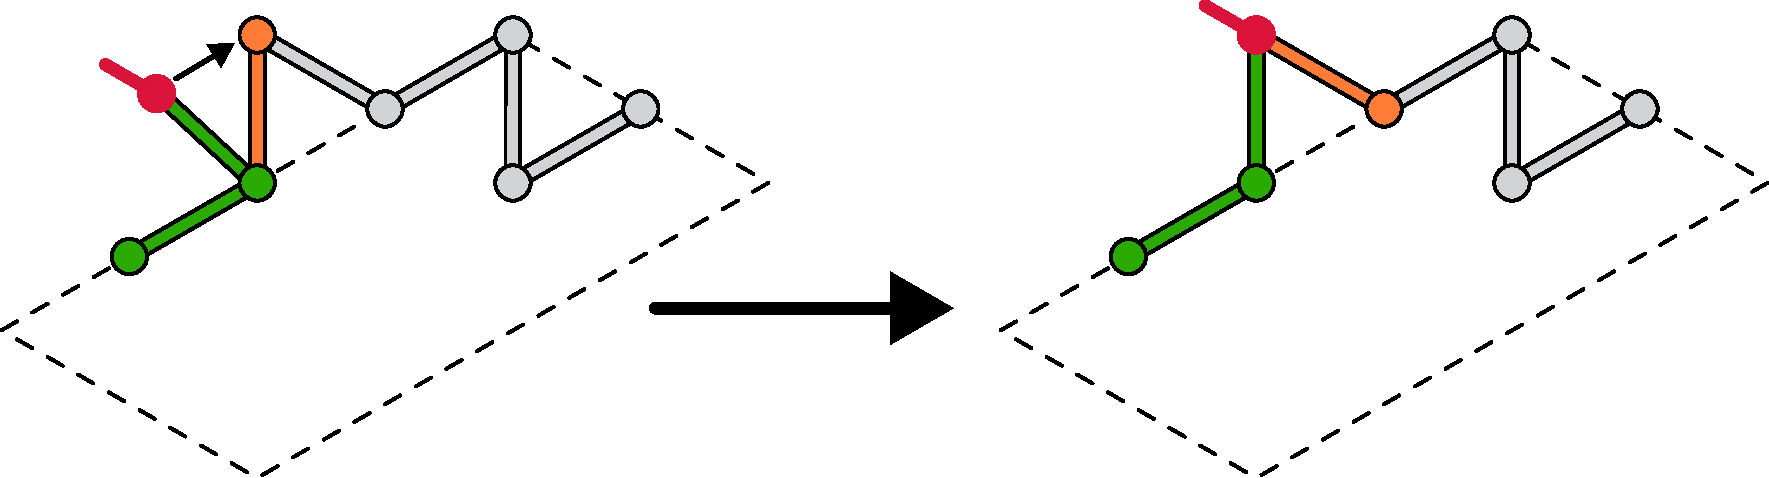
\includegraphics[width=0.8\linewidth]{./implementation/figures/task-example.pdf}
\end{figureBox}

Participants have a time limit of one minute to complete each task. The time at which each point is completed, as well as the position of the hand and eye throughout the task, is recorded. If participants do not complete the task within the time limit, the task is marked as incomplete, and all completed segments are logged. The five different tasks are shown in Fig~\ref{fig:tasks}.

\begin{figureBox}[label={fig:tasks}, width=1.0\linewidth]{The Five Tasks}
    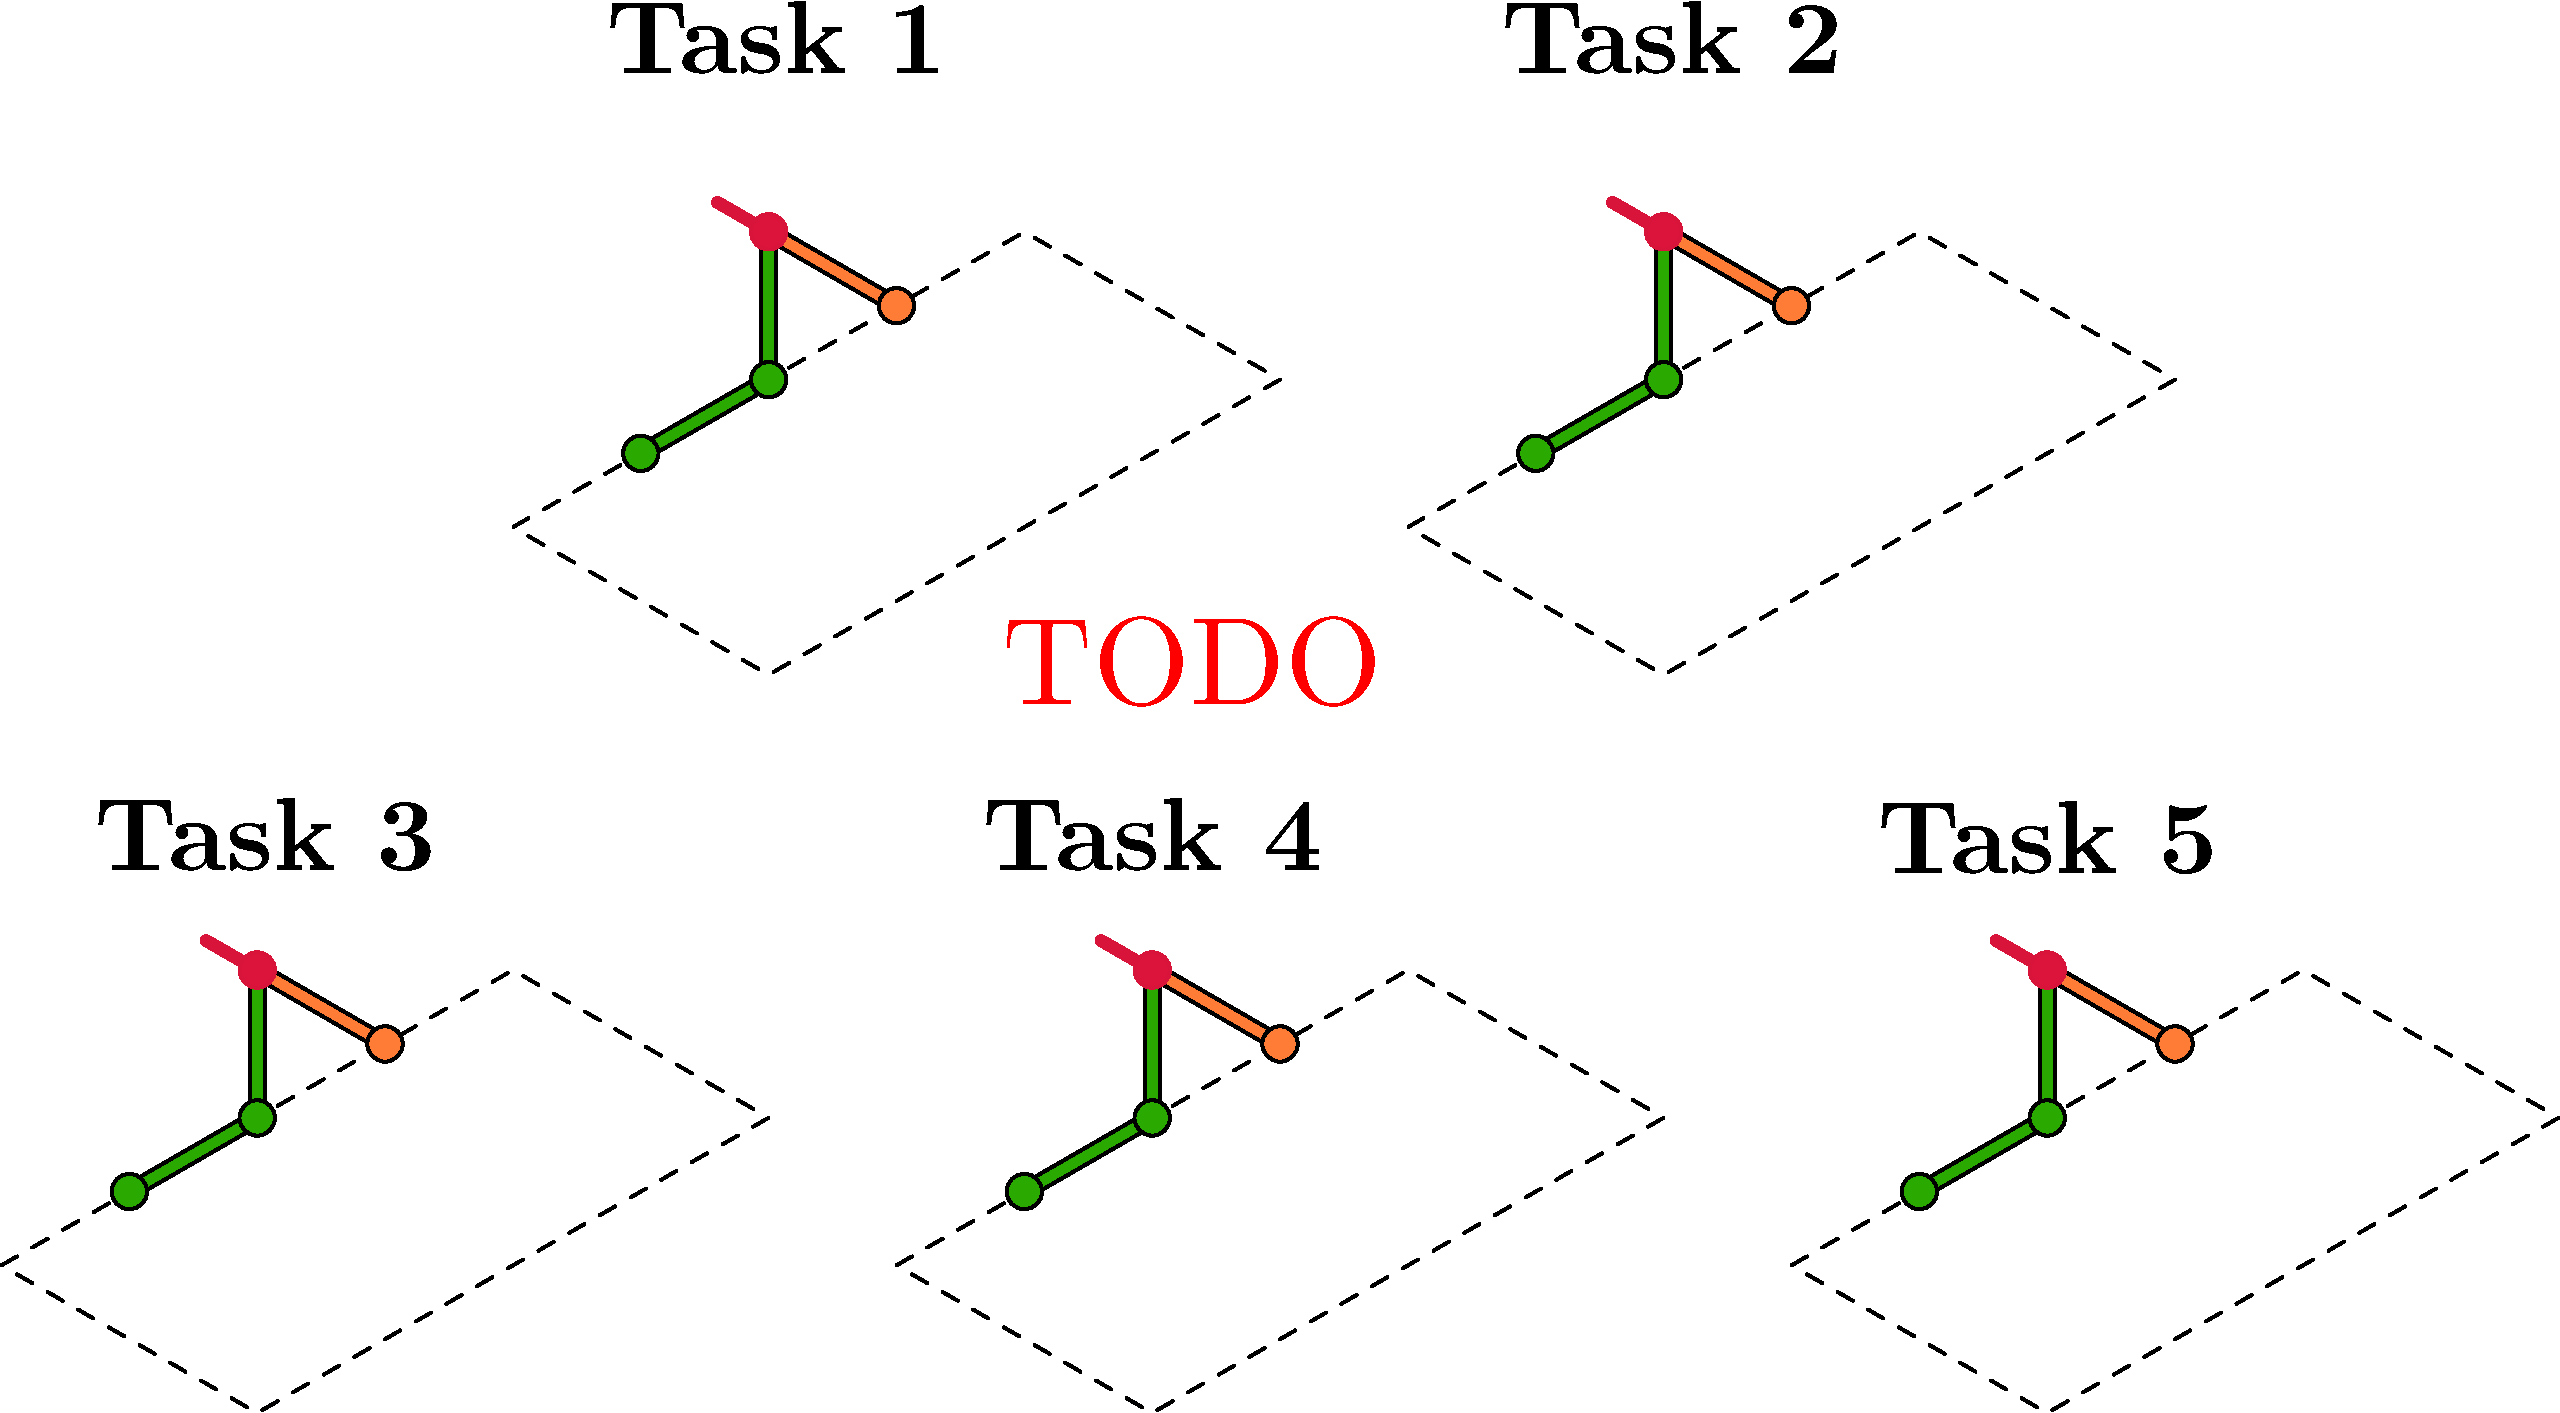
\includegraphics[width=0.8\linewidth]{./implementation/figures/tasks.pdf}
\end{figureBox}

Participants are also given two demonstration tasks to familiarize themselves with the system, as seen in Fig~\ref{fig:demo-conditions}.

\begin{figureBox}[label={fig:demo-conditions}, width=0.8\linewidth]{Demo Conditions}
    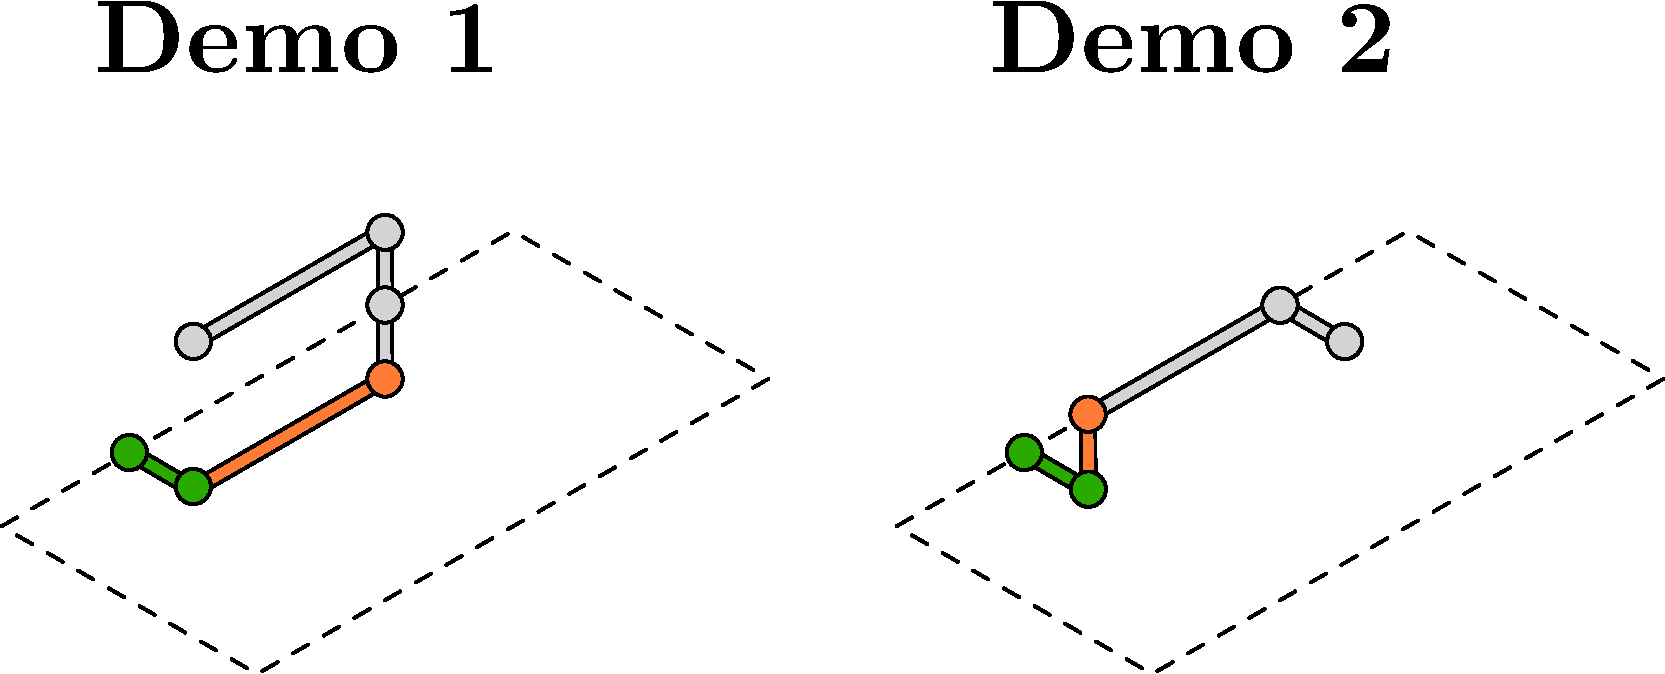
\includegraphics[width=0.65\linewidth]{./implementation/figures/demos.pdf}
\end{figureBox}


\subsection{Participants}

Participants were recruited for the study via email and text message using a standardized script to ensure the process was unbiased. Upon arrival, participants were required to fill out a consent form and complete the first page of a questionnaire. This initial questionnaire collected demographic and personal information that could influence the study results, such as age, handedness, previous experience with VR/AR, and whether they wore glasses (the full questionnaire is provided in the appendix). \\

Following this, participants received a brief overview of the system and had the opportunity to run through two demo tasks in each of the four different configurations to familiarize themselves with the system. Participants were instructed to keep their non-dominant hand on their lap and place their dominant hand face down on the monitor at the start of each task to facilitate tracking. They were permitted to repeat the demo tasks up to three times if necessary. \\

Once the participants felt comfortable with the system, they were entered into the study's system and were automatically assigned a random sequence of the four experimental conditions, as shown in Figure~\ref{fig:study-conditions}.

\begin{figureBox}[label={fig:study-conditions}, width=0.8\linewidth]{Study Conditions}
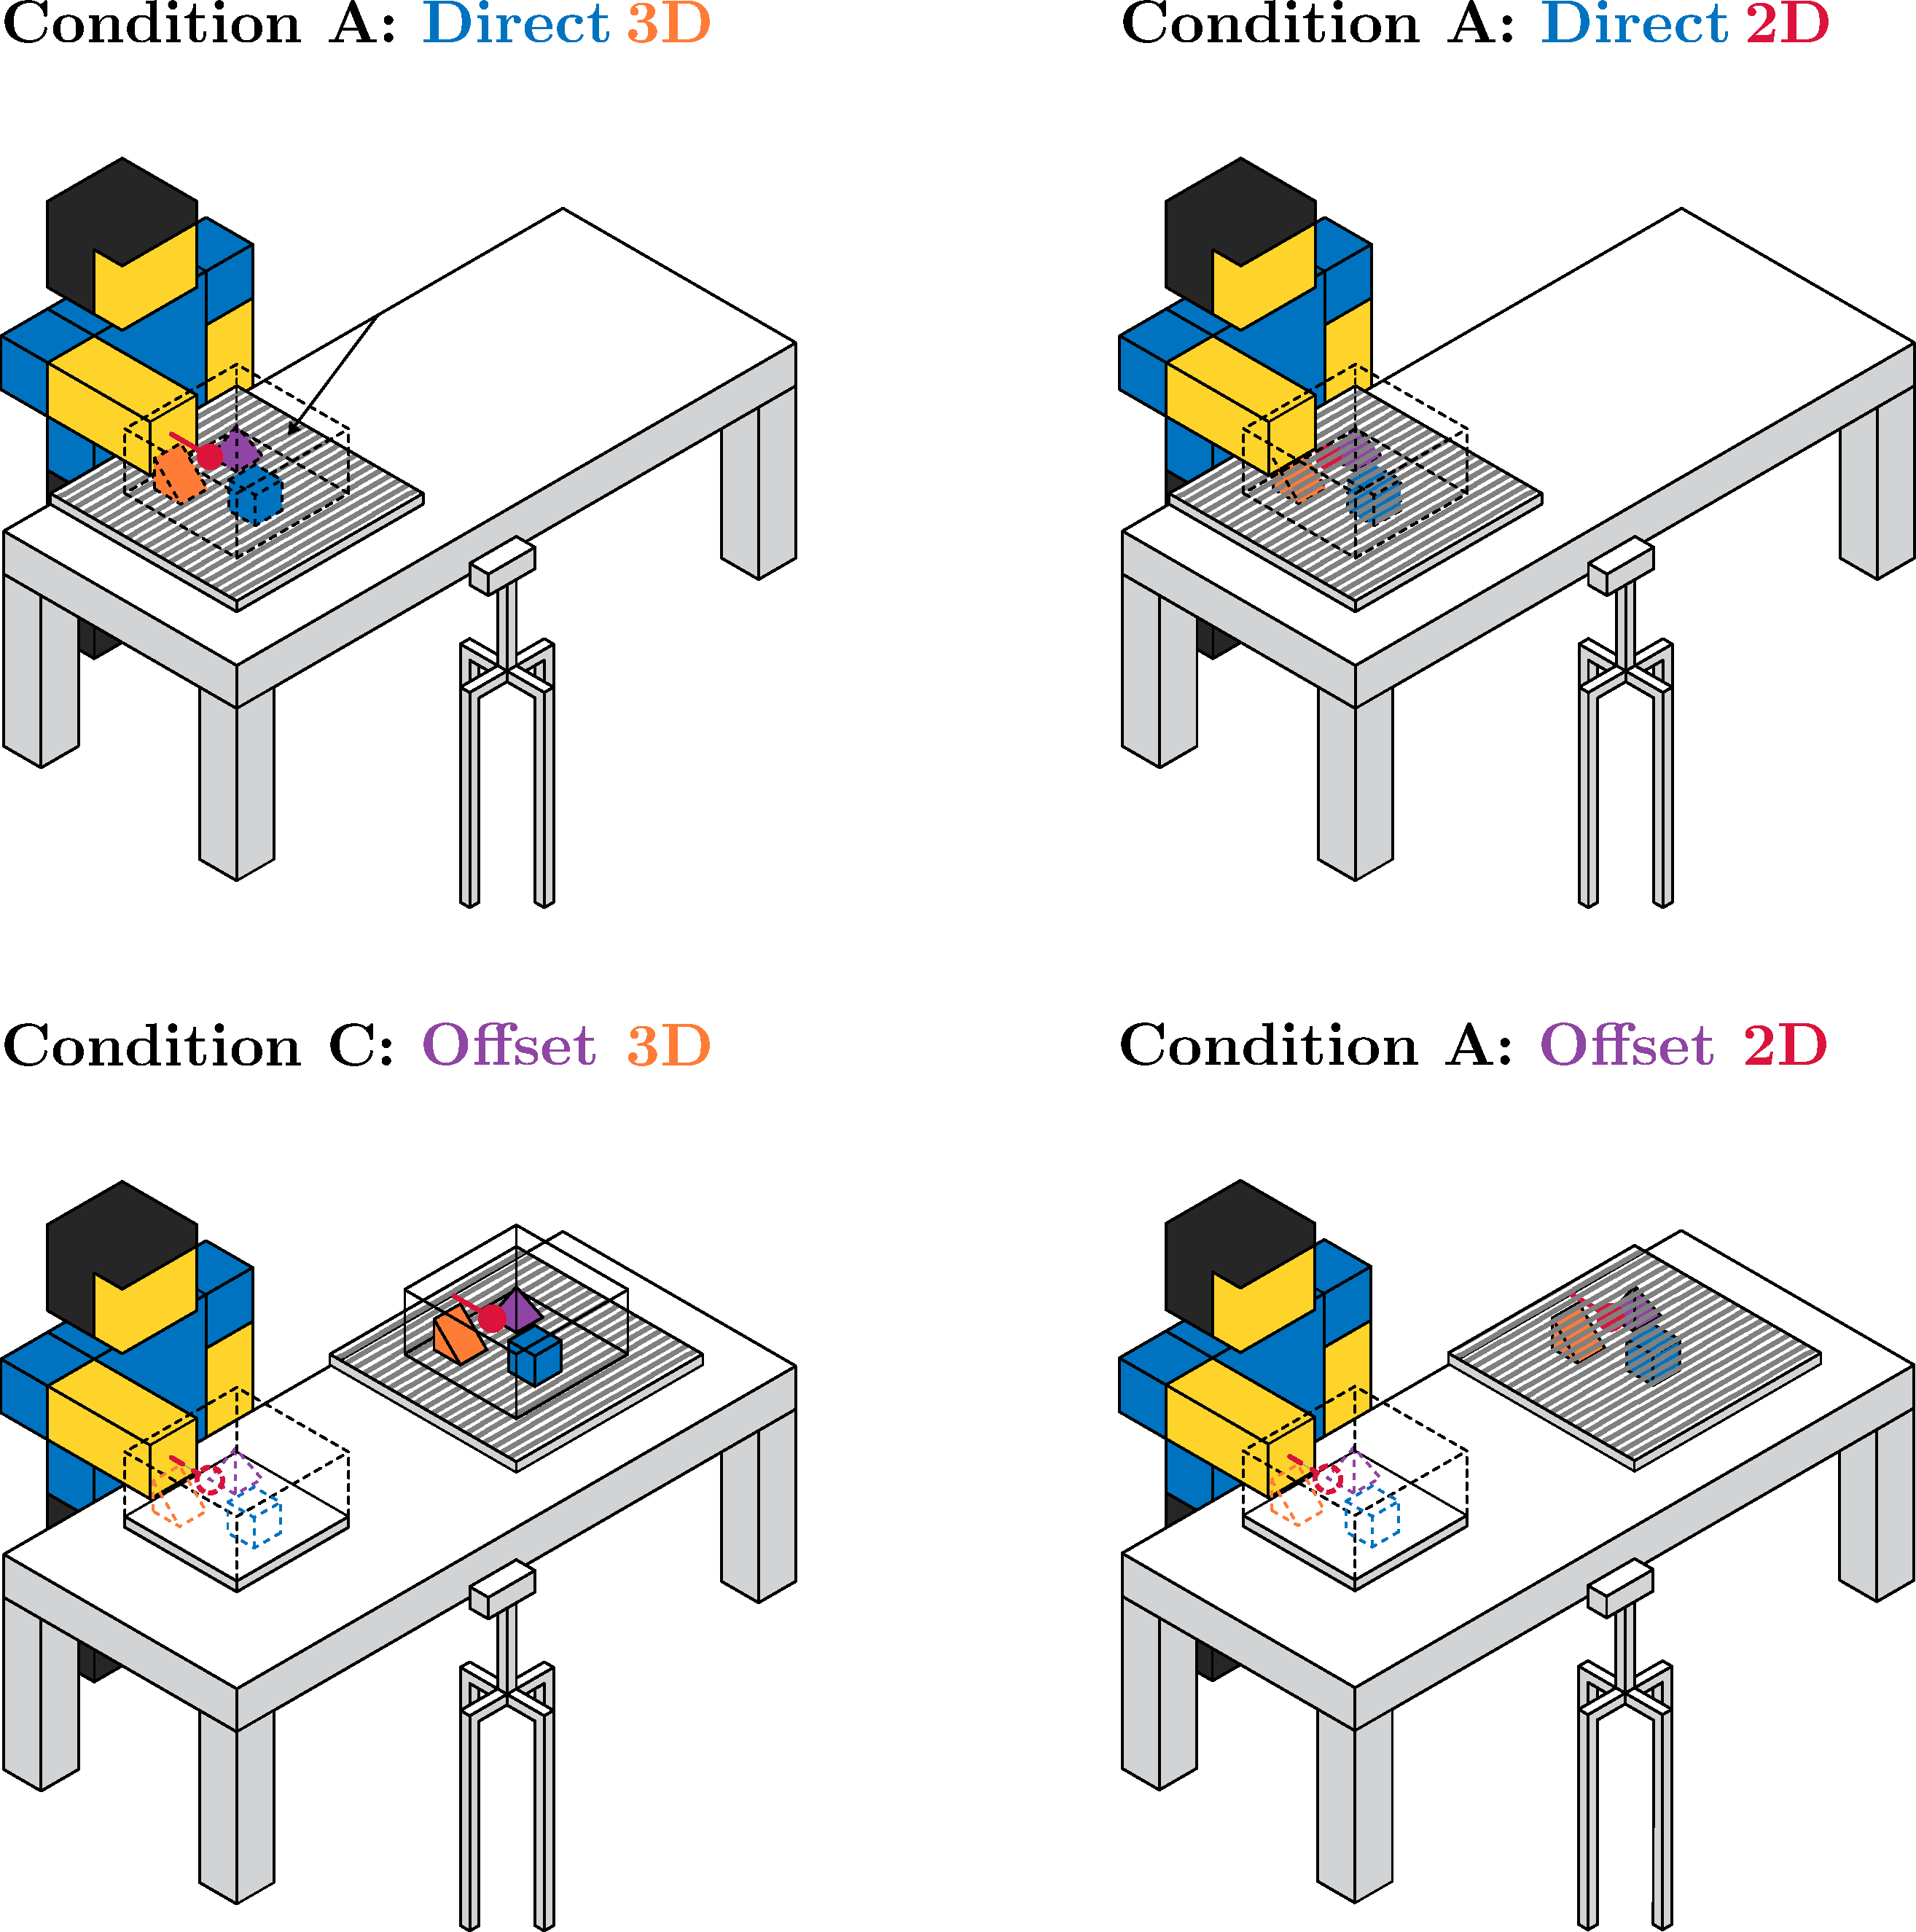
\includegraphics[width = 0.8\linewidth]{./implementation/figures/study-conditions.pdf}
\end{figureBox}

Each condition comprised five tasks, each lasting one minute, which participants were required to complete sequentially. An audio cue signaled the start and end of each task. Participants were allowed to take breaks between conditions. After completing each condition, they filled out a survey regarding that condition. At the end of the study, they completed a survey about the overall system. Both surveys are included in the appendix.
\subsection{Setup}

The study was conducted on the ground floor of the Huxley building in Room 218 at Imperial College London's South Kensington Campus. Considering that the study would span multiple days, we took special care to set up the system to minimize the risk of accidental changes to the setup. As depicted in Fig~\ref{fig:front-view-study}, the camera was mounted on a tripod, and the positions of the tripod legs were marked on the floor to maintain consistency. Additionally, we surrounded the camera with a barrier of tables to prevent it from being knocked over.

\begin{invisBox}
	\pictureBox[label={fig:front-view-study}]{Study: Front View}{
		\adjustbox{height=5cm, keepaspectratio}{
			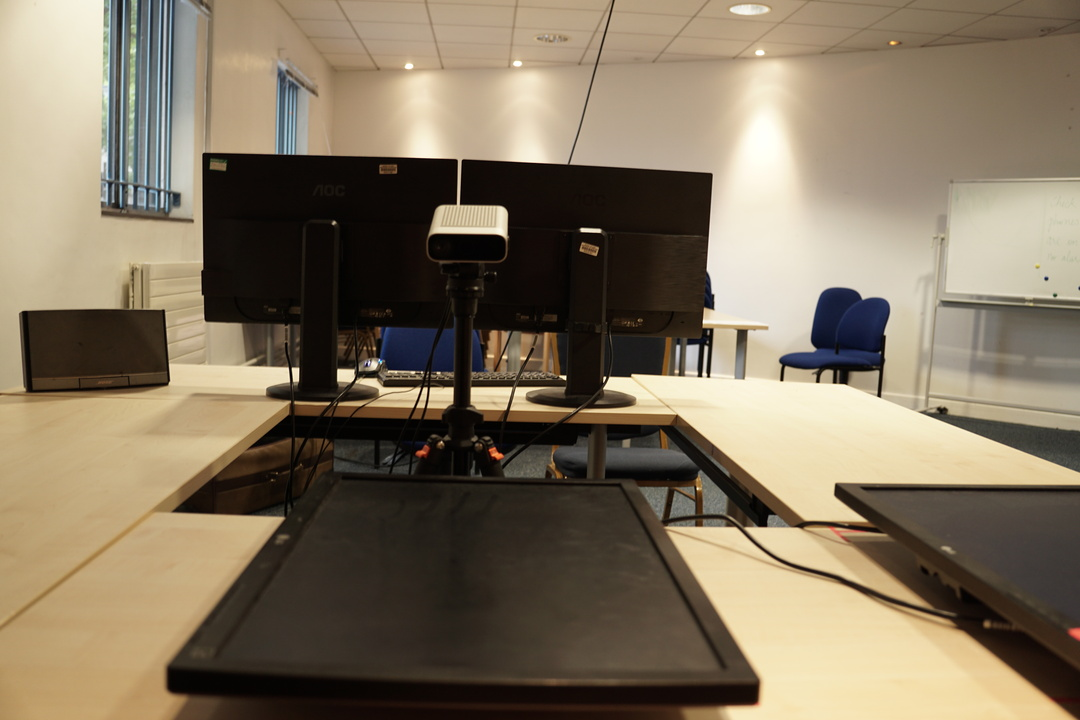
\includegraphics{./implementation/figures/front-view.jpg}
		}
	}
	\hfill
	\pictureBox[label={fig:side-view-study}]{Study: Side View}{
		\adjustbox{height=5cm, keepaspectratio}{
			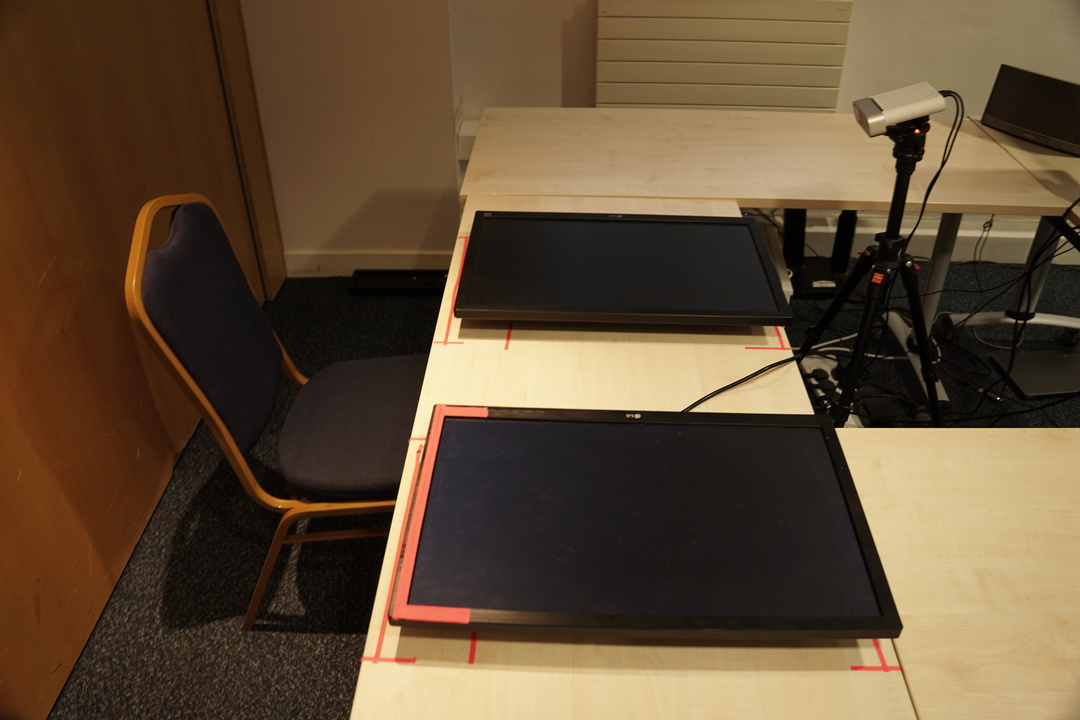
\includegraphics{./implementation/figures/side-view.jpg}
		}
	}
\end{invisBox}

The displays used for the study were $24''$ $1920 \times 1200$ \texttt{LG IPS LED 24EB23} computer monitors, which were detached from their stands and placed horizontally on a table. There was a 25 cm gap between the bottom of the farther monitor and the top of the closer monitor, as shown in Fig~\ref{fig:side-view-study}.

The camera was positioned such that the user’s head was approximately 1 meter away, although this distance varied slightly with participant height. The interaction zone on the far display was set up such that participants interacted with the scene at distances ranging from 30 to 70 cm from the camera. These distances were selected to fall within the optimal tracking range of our system (discussed in more detail in the evaluation section).

To facilitate the study and monitor participants effectively, we set up two additional monitors opposite the participants, as shown in Fig~\ref{fig:control-view-study}. These monitors allowed the study conductor to control the system and observe the participants. Using large monitors helped to block the view of the study conductor, thereby reducing the possibility of participants feeling observed, which might introduce unintended bias.

\begin{invisBox}
	\pictureBox[label={fig:control-view-study}]{Study: Control View}{
		\adjustbox{height=5cm, keepaspectratio}{
			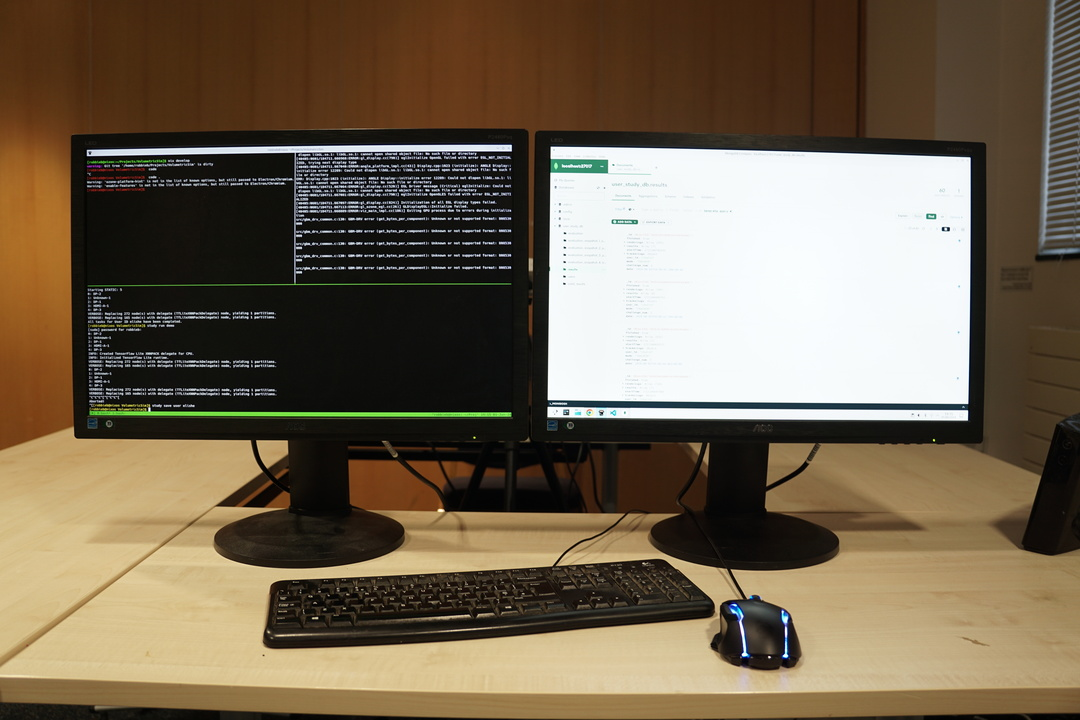
\includegraphics{./implementation/figures/control-view.jpg}
		}
	}
	\hfill
	\pictureBox[label={fig:calibration-device-study}]{Study: Calibration Device}{
		\adjustbox{height=5cm, keepaspectratio}{
			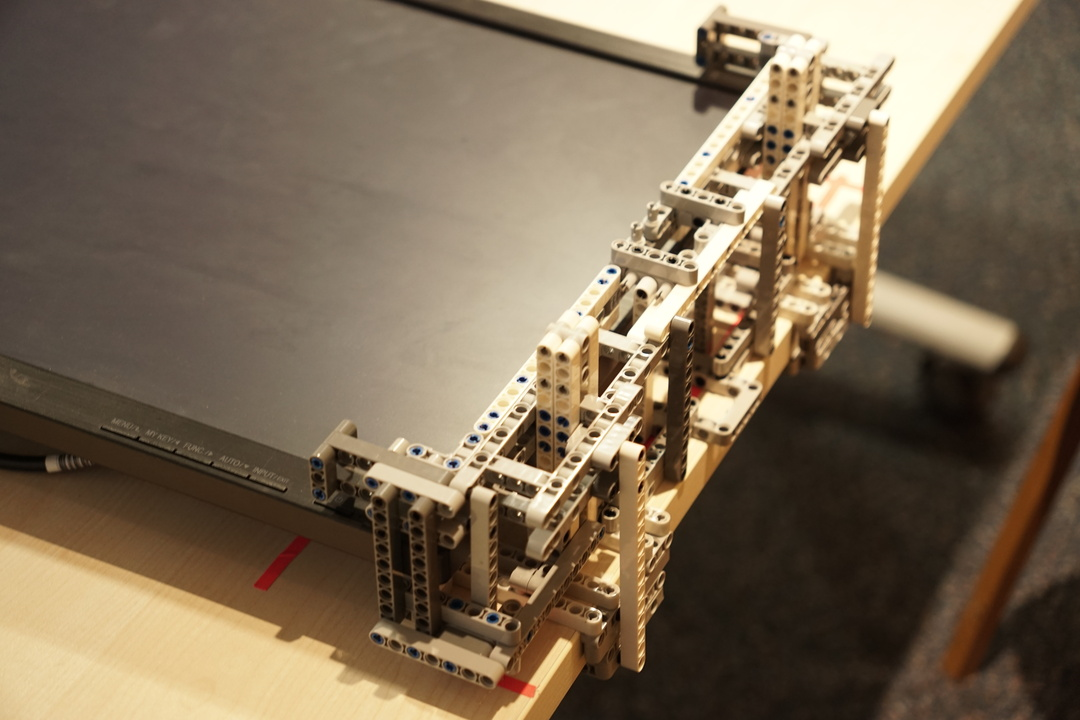
\includegraphics{./implementation/figures/calibration-device.jpg}
		}
	}
\end{invisBox}

We also designed and built a calibration device to realign the displays after each participant completed their tasks, as depicted in Fig~\ref{fig:calibration-device-study}. Participants often inadvertently moved the displays during the tasks, and this simple device, made from Lego Technic (A line of Lego interconnecting plastic rods and parts, which is useful for creating a variety of mechanical systems), enabled us to easily and accurately reposition the displays to their original alignment.

\subsection{Evaluation Metrics and Collected Data}

The evaluation of the system was based on two primary metrics: the time taken to complete each task and the number of subtasks completed within the designated time frame. For precise measurement, a time stamp was recorded at the beginning of each task and at the completion of each subtask. This allowed us to accurately track task duration and identify any performance patterns. Additionally, we monitored and recorded instances of tracking failures to ensure that we could filter out erroneous data during the analysis phase, thus maintaining the integrity of our results. \\

Throughout each task, we continuously logged the positions of the participants' eyes, middle fingers, and index fingers, along with corresponding time stamps. This comprehensive data collection enabled a detailed analysis of participant movements and interactions. Specifically, the logged data allowed us to plot the paths taken by participants, which provided valuable insights into their interaction patterns. An example of such a plot is shown in Fig~\ref{fig:finger-trace}, illustrating the trajectory of a user's finger movements during Task 4.

\begin{figureBox}[label={fig:finger-trace}, width=0.8\linewidth]{Example of logging a user's path for Task 4}
    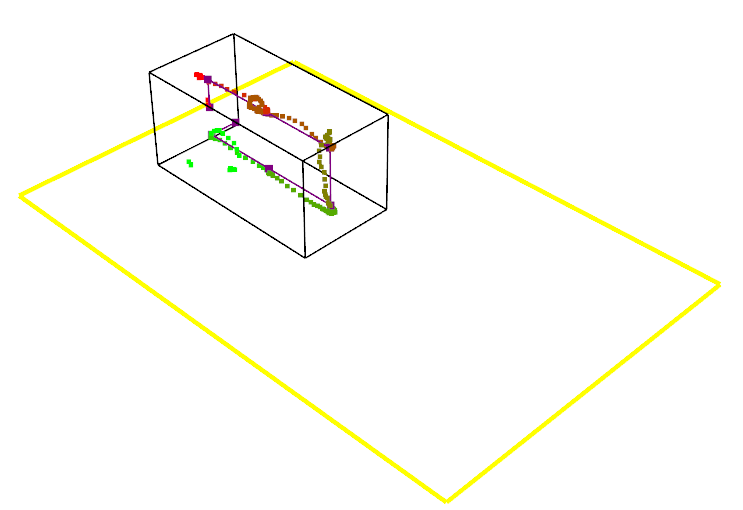
\includegraphics[width = 0.8\linewidth]{./implementation/figures/finger-trace-plot.png}
\end{figureBox}

To ensure comprehensive evaluation, we also collected additional data points such as error rates, which included the frequency and types of errors participants made during the tasks. This data provided deeper insights into the usability and reliability of the system. Moreover, participant feedback was collected through post-task and post-condition surveys, offering qualitative data that complemented the quantitative metrics. This holistic approach ensured that we could thoroughly assess both the performance and user experience aspects of the system.

\subsection{Study Implementation}

The study was run from a python based CLI using the Click \cite{noauthor_palletsclick_2024} library. To make the study experience as seamless as possible, we designed a user-friendly CLI interface that guided study runner through the study process. The CLI would automatically start the next task with a simple one line command as can be seen in List~\ref{list:study-cli}.

\codeBoxFile[label = {list:study-cli},  width=0.75\linewidth]{shell}{./implementation/code/study-cli.sh}{Terminal}
